Este capítulo describe las técnicas de análisis implementadas en la aplicación, las variables utilizadas y los resultados que generan. Se distinguen dos grupos de procedimientos: por una parte, indicadores heurísticos construidos mediante agregaciones, reglas y ponderaciones definidas específicamente para el proyecto; por otra, modelos de aprendizaje automático y una simulación probabilística. Los scripts se encuentran en el directorio \path{DATA_MINING/SCRIPTS/} y sus salidas se almacenan en \path{DATA_MINING/DSA_DM/}.

\section{Métricas e indicadores estadísticos}

Los indicadores de este apartado no son modelos de aprendizaje automático. Se calculan mediante reglas deterministas que agregan, normalizan y ponderan las estadísticas disponibles. Su finalidad es resumir la información deportiva y facilitar su interpretación dentro de la aplicación.

\subsection{Índice de forma de un jugador}

El índice de forma de los jugadores se implementa en el script \path{estado_forma_jugador.py} y se calcula para la temporada 2025. El procedimiento parte de las estadísticas de cada futbolista por partido y construye primero una puntuación individual:

\begin{equation}
    S_{partido}=0.6\,N+0.4\,A,
\end{equation}

donde $N$ es la valoración del jugador proporcionada por la fuente de datos y $A$ representa una suma ponderada de sus acciones. Todos los jugadores reciben puntuación por goles y asistencias; además, se aplican contribuciones específicas según su posición. Por ejemplo, los defensas reciben puntuación por entradas e intercepciones y son penalizados por regates recibidos y goles concedidos, mientras que los porteros reciben puntuación por paradas y penaltis detenidos y son penalizados por los goles encajados.

La puntuación de la temporada se obtiene como la media de los encuentros en los que el jugador ha disputado al menos 15 minutos. Para calcular la forma reciente, se consideran sus siete apariciones más recientes y se conservan aquellas en las que ha jugado al menos 20 minutos. Si quedan menos de tres partidos válidos, el estado se clasifica como \textit{Pocos minutos}. En caso contrario, la evolución se define como:

\begin{equation}
    E=S_{reciente}-S_{temporada}.
\end{equation}

El jugador se clasifica con \textit{Rendimiento alto} cuando $E>0.3$, con \textit{Rendimiento bajo} cuando $E<-0.3$ y como \textit{Estable} en el resto de los casos. El resultado se almacena en \path{ESTADO_FORMA_JUGADORES_2025.csv}, junto con las puntuaciones de temporada y de forma reciente.

Este indicador permite detectar cambios recientes respecto al rendimiento medio del propio jugador. No constituye una valoración absoluta de su calidad ni una predicción de su rendimiento futuro.

\subsection{Índice de forma de un equipo}

El índice de forma de los equipos se implementa en \path{estado_forma_equipo.py}. Para cada equipo se seleccionan los cinco partidos más recientes y se asignan inicialmente 3 puntos por victoria, 1 por empate y 0 por derrota. Esta puntuación se ajusta utilizando los goles esperados del encuentro y la dificultad del rival. En particular, se añade un bono de 0.5 puntos cuando el rival pertenece a los seis primeros puestos de la clasificación tomada como referencia.

Los partidos más recientes reciben mayor importancia mediante una ponderación exponencial. Si los encuentros se ordenan del más antiguo al más reciente, sus pesos son $0.85^4$, $0.85^3$, $0.85^2$, $0.85$ y $1$. La media ponderada se normaliza posteriormente sobre una escala de 0 a 10:

\begin{equation}
    S_{equipo}=\min\left(10,\frac{10}{3}\frac{\sum_i w_i p_i}{\sum_i w_i}\right),
\end{equation}

donde $p_i$ es la puntuación ajustada de cada partido y $w_i$ su peso temporal. El estado se considera \textit{Positivo} cuando la nota es igual o superior a 5.5, \textit{Estable} cuando se encuentra entre 3.2 y 5.5, y \textit{Crítico} cuando es inferior a 3.2.

El script también almacena la media ponderada y la desviación estándar de las puntuaciones ponderadas en los campos \texttt{tendencia} y \texttt{variabilidad}, respectivamente. Estas medidas resumen el nivel reciente y su dispersión, pero no representan una tendencia temporal estimada mediante regresión.

\subsection{Análisis de necesidades de plantilla}

El script \path{aspectos_a_mejorar.py} identifica posibles posiciones que convendría reforzar. Para ello, agrega las estadísticas de los jugadores por equipo, temporada y posición, calcula tasas por 90 minutos y compara cada equipo con la media de la competición para esa misma temporada y posición.

Una métrica se considera baja cuando se encuentra al menos un 10\% por debajo de la media y alta cuando la supera, como mínimo, en un 10\%. Las reglas aplicadas se resumen en la Tabla~\ref{tab:criterios_necesidades}.

\begin{table}[H]
\centering
\caption{Criterios utilizados para detectar necesidades de plantilla.}
\label{tab:criterios_necesidades}
\begin{tabular}{|p{2.5cm}|p{4.7cm}|p{5.7cm}|}
\hline
\textbf{Necesidad} & \textbf{Indicadores analizados} & \textbf{Condición general} \\
\hline
Delantero & Goles a favor del equipo & Valor inferior a la media de la liga. \\
\hline
Extremo & Tasa de regates completados y asistencias por 90 minutos de los delanteros & Ambos valores inferiores a la media de la posición. \\
\hline
Medio ofensivo & Precisión de pase, pases clave y asistencias por 90 minutos de los mediocentros & Los tres valores inferiores a la media de la posición. \\
\hline
Pivote defensivo & Faltas, precisión de pase e intercepciones por 90 minutos de los mediocentros & Faltas superiores a la media y precisión e intercepciones inferiores. \\
\hline
Laterales & Asistencias y regates recibidos por 90 minutos de los defensas & Pocas asistencias y más regates recibidos que la media. \\
\hline
Central & Goles encajados, entradas, bloqueos e intercepciones por 90 minutos & Goles encajados superiores a la media y métricas defensivas inferiores. \\
\hline
Portero & Paradas y goles concedidos por 90 minutos & Menos paradas y más goles concedidos que la media. \\
\hline
\end{tabular}
\end{table}

Si no se cumple ninguna regla, el resultado indica que no existe una necesidad clara. Se trata de un sistema heurístico de apoyo: las asociaciones anteriores no demuestran por sí mismas que una posición sea la causa del rendimiento del equipo.

\subsection{Perfil estadístico de un jugador}

El script \path{ratings.py} transforma las estadísticas acumuladas de cada jugador en seis dimensiones: ataque, creación, defensa, portería, duelos y regates. Cada dimensión combina variables relacionadas con ese aspecto del juego. Por ejemplo, ataque utiliza goles y tiros a puerta; creación emplea pases, pases clave, asistencias y precisión; y defensa considera entradas, intercepciones, bloqueos y determinadas penalizaciones disciplinarias.

Para reducir el efecto de muestras pequeñas se aplica un factor de experiencia definido como:

\begin{equation}
    F_{experiencia}=\min\left(1,\frac{partidos}{10}\right).
\end{equation}

Las seis puntuaciones se calculan por jugador y temporada. Después se normalizan de forma independiente dentro de cada temporada, asignando el valor 10 al máximo observado en cada dimensión y escalando proporcionalmente el resto. También se calcula el percentil del jugador respecto a los demás futbolistas de esa campaña.

El resultado se guarda en \path{perfil_estadistico_jugadores.csv}. Estas puntuaciones son índices internos de la aplicación y no deben interpretarse como escalas universales o directamente comparables con valoraciones de otras fuentes.

\subsection{Recomendador de fichajes}

El recomendador se implementa en \path{recomendacion_fichajes_refuerzo.py}. Combina las necesidades de plantilla, los perfiles estadísticos, los grupos obtenidos mediante \textit{K-means}, las estadísticas por temporada, la clasificación de los equipos, la edad y el estado de forma reciente de los jugadores.

Primero se selecciona la temporada más reciente común a todas las fuentes y se consolidan las necesidades que corresponden a una misma posición general. Después se descartan los futbolistas con menos de 600 minutos y los que pertenecen al propio equipo. Los clubes se distribuyen en cuatro tramos según su posición: 1--3, 4--7, 8--14 y 15--20. Un club solo recibe candidatos procedentes de su mismo tramo o de uno inferior. También se excluyen cuatro parejas de clubes rivales definidas explícitamente en el script.

Para cada necesidad se identifica el clúster con mayor puntuación media en los atributos relevantes. Dentro de ese grupo se construye un perfil objetivo a partir del cuartil superior de jugadores. La similitud de cada candidato con dicho perfil se calcula mediante similitud coseno después de estandarizar las seis dimensiones estadísticas.

La puntuación final combina los siguientes factores:

\begin{itemize}
    \item Similitud con el perfil objetivo: 40\%;
    \item Nota media de la temporada: 25\%;
    \item Estado de forma reciente: 15\%;
    \item Edad: 10\%;
    \item Experiencia, medida mediante partidos disputados: 10\%.
\end{itemize}

La puntuación de edad alcanza su máximo en los 23,5 años, punto medio del intervalo ideal definido entre 20 y 27 años, y disminuye linealmente al alejarse de ese valor. Finalmente, se devuelven como máximo tres candidatos por necesidad. El resultado es determinista y explicable, pero no incorpora precio, duración del contrato, salario, lesiones ni disponibilidad real en el mercado; por tanto, debe entenderse como una recomendación estadística preliminar.

\subsection{Indicador de posibles goleadores}

El script \path{prob_goleadores.py} ordena a los jugadores de cada equipo según su propensión estimada a marcar en los partidos pendientes. Para cada futbolista, combina la media de goles de sus siete apariciones más recientes, su promedio goleador en la temporada 2025 y los goles anotados históricamente contra el rival:

\begin{equation}
    z=0.35\,G_{reciente}+0.45\,G_{temporada}+0.05\,\min(G_{rival},3).
\end{equation}

El valor se transforma mediante una función sigmoide, $p=1/(1+e^{-2(z-0.5)})$, y se limita a un máximo de 0.75. Para cada partido se seleccionan los tres jugadores con mayor valor de cada equipo.

Aunque el campo de salida se denomina \texttt{probabilidad}, el valor no ha sido calibrado contra frecuencias observadas. En consecuencia, debe interpretarse como un indicador heurístico para ordenar candidatos y no como una probabilidad estadística validada de marcar.

\section{Técnicas de minería de datos y aprendizaje automático}

\subsection{Jugadores similares mediante \textit{K-means}}

\textit{K-means} es una técnica de aprendizaje no supervisado que agrupa observaciones tratando de minimizar la distancia cuadrática respecto al centroide de su clúster \cite{azzami_clustering_2025}. En este proyecto se utiliza como primera etapa para reducir el conjunto de candidatos con perfiles estadísticos próximos.

\begin{figure}[H]
    \centering
    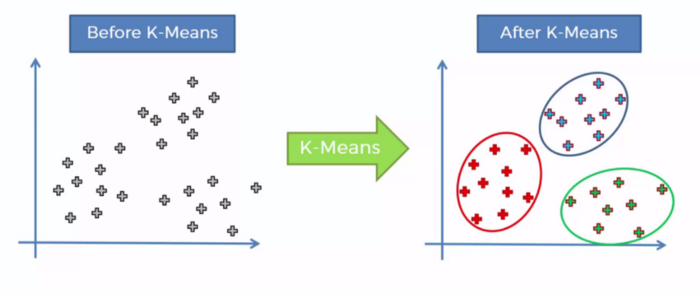
\includegraphics[width=0.7\linewidth]{figures/kmeans.png}
    \caption{Representación del funcionamiento de \textit{K-means}.}
    \label{fig:kmeans}
\end{figure}

\subsubsection{Implementación}

La implementación se encuentra en \path{similitud_jugadores.py} y utiliza como entrada \path{perfil_estadistico_jugadores.csv}. Las variables son ataque, creación, defensa, portería, duelos y regates. Los valores ausentes se sustituyen por la mediana y las variables se estandarizan mediante puntuaciones $z$ para evitar que su escala determine las distancias.

El proceso se ejecuta de forma independiente para cada temporada. El número de clústeres se calcula mediante $\lfloor\sqrt{n/2}\rfloor$, con un mínimo de 2 y un máximo de 20 cuando existen al menos tres jugadores. Se realizan cinco inicializaciones con semilla reproducible y se conserva la solución con menor inercia. Cada ejecución admite un máximo de 100 iteraciones.

Una vez asignados los clústeres, la similitud final se calcula mediante el coseno entre los perfiles estandarizados. Para cada jugador se buscan primero futbolistas de la misma posición y del mismo clúster. Si no existen cinco candidatos, la lista se completa con jugadores de la misma posición pertenecientes a otros clústeres. Por tanto, \textit{K-means} realiza la agrupación inicial, mientras que la similitud coseno determina el orden final de los cinco jugadores más parecidos.

\subsection{Predicción de partidos mediante clasificación supervisada}

El script \path{predicccion.py} plantea la predicción como un problema multiclase con tres resultados: victoria local, empate y victoria visitante. Se comparan Random Forest, Gradient Boosting y una máquina de vectores soporte (SVM) con núcleo RBF.

Para cada equipo se calculan, utilizando únicamente encuentros anteriores a la fecha del partido, las medias de puntos, goles a favor y goles en contra durante los últimos 5 y 10 partidos. También se obtienen las mismas variables restringidas a la condición de local o visitante. A estas características se añaden estadísticas acumuladas de temporada, como posición, puntos, diferencia de goles, victorias, empates, derrotas y resultados desglosados por localía.

Los partidos completados se ordenan cronológicamente. El 80\% inicial se utiliza para entrenamiento y el 20\% final para validación. Los valores ausentes se sustituyen por la mediana del conjunto de entrenamiento. En el caso de SVM, las variables se estandarizan antes de ajustar el modelo.

\subsubsection{Evaluación de los modelos}

Se emplean las métricas \textit{accuracy}, precisión macro, \textit{recall} macro y F1 macro. La F1 macro concede el mismo peso a las tres clases y resulta útil porque el empate suele estar peor representado que las victorias locales o visitantes.

\begin{table}[H]
\centering
\caption{Comparación de modelos para la predicción de partidos.}
\label{tab:evaluacion_prediccion}
\begin{tabular}{|l|c|c|c|c|}
\hline
\textbf{Modelo} & \textbf{Accuracy} & \textbf{Precisión macro} & \textbf{Recall macro} & \textbf{F1 macro} \\
\hline
SVM & 0.5586 & 0.5593 & 0.5527 & 0.5464 \\
\hline
Random forest & 0.5698 & 0.5464 & 0.5376 & 0.5385 \\
\hline
Gradient boosting & 0.5599 & 0.5446 & 0.5338 & 0.5311 \\
\hline
\end{tabular}
\end{table}

Random Forest obtiene la mayor tasa global de acierto, con un 56,98\%. Sin embargo, SVM alcanza la mejor F1 macro, con 0,5464, por lo que se utiliza para generar las predicciones de los partidos pendientes. El modelo se vuelve a entrenar con todos los partidos completados y produce las probabilidades de victoria local, empate y victoria visitante que consume posteriormente la simulación de Monte Carlo.

Las probabilidades proceden de la estimación interna habilitada por \texttt{SVC (probability=True)}. No se ha realizado una calibración externa adicional, por lo que deben interpretarse con cautela.

\subsection{Probabilidades de clasificación mediante simulación de Monte Carlo}

La simulación de Monte Carlo permite aproximar la distribución de resultados de un sistema mediante la repetición de escenarios aleatorios \cite{stock_physics-based_2022}. En este proyecto se utiliza para estimar la posición final de los equipos a partir de la clasificación actual y de las probabilidades 1X2 generadas por SVM.

El script \path{simulacion_montecarlo_laliga.py} ejecuta 10.000 simulaciones con semilla 42. En cada partido pendiente se genera un número aleatorio y se asigna una victoria local, un empate o una victoria visitante según las probabilidades correspondientes. A continuación se actualizan los puntos de ambos equipos.

Para aproximar el desempate, cada victoria simulada modifica la diferencia de goles $+1$ para el vencedor y $-1$ para el derrotado; los empates no la alteran. Si dos equipos continúan igualados a puntos y diferencia de goles, se ordenan por nombre. Esta simplificación permite generar una clasificación completa, aunque no reproduce todos los criterios oficiales de desempate ni simula marcadores exactos.

Al finalizar cada iteración se registran las siguientes categorías: campeón, puestos 1--4, puestos 5--7, puestos 8--17 y descenso, correspondiente a las posiciones 18--20. Las frecuencias obtenidas tras las 10.000 iteraciones se presentan como porcentajes estimados.

\subsection{Estimación de goles mediante regresión}

El script \path{prediccion_goles_partidos.py} complementa la predicción 1X2 estimando dos valores continuos: los goles del equipo local y los goles del visitante. Se emplean las mismas características recientes y acumuladas que en el modelo de clasificación.

Se comparan Random Forest Regressor, Gradient Boosting Regressor, Support Vector Regression y una red neuronal MLP. La evaluación utiliza la misma división temporal 80/20. Los valores predichos se limitan inferiormente a cero y se calculan el error absoluto medio (MAE), la raíz del error cuadrático medio (RMSE) y el coeficiente de determinación ($R^2$).

\begin{table}[H]
\centering
\caption{Comparación de modelos para la estimación de goles.}
\label{tab:evaluacion_goles_estimados}
\begin{tabular}{|l|c|c|c|}
\hline
\textbf{Modelo} & \textbf{MAE} & \textbf{RMSE} & \textbf{$R^2$} \\
\hline
Random Forest Regressor & 0.8237 & 1.0663 & 0.1791 \\
\hline
MLP Regressor & 0.8647 & 1.1016 & 0.1239 \\
\hline
SVR & 0.8844 & 1.1627 & 0.0240 \\
\hline
Gradient Boosting Regressor & 0.9063 & 1.1716 & 0.0091 \\
\hline
\end{tabular}
\end{table}

Random Forest Regressor obtiene el menor MAE y RMSE y el mayor$R^2$, por lo que se selecciona como modelo final. Un MAE de 0.8237 indica un error absoluto medio ligeramente inferior a un gol por equipo y partido. No obstante, el $R^2$ de 0.1791 muestra que el modelo explica una proporción reducida de la variabilidad de los marcadores.

La salida incluye los goles estimados de ambos equipos, su diferencia, un resultado 1X2 derivado y un marcador obtenido mediante redondeo. Estos valores no representan la métrica convencional de goles esperados o xG basada en la calidad de cada ocasión, sino una predicción agregada de goles a partir del historial de los equipos.

\section{Limitaciones metodológicas}

Los resultados presentados deben interpretarse dentro del alcance académico del proyecto. Los indicadores de forma, necesidades de plantilla, recomendación de fichajes y posibles goleadores se basan en reglas y ponderaciones diseñadas para la aplicación; no han sido validados mediante estudios con clubes, analistas o usuarios expertos.

Además, aunque las características recientes de los modelos predictivos se calculan utilizando partidos anteriores a cada encuentro, la implementación incorpora a todos los partidos de una temporada la última instantánea disponible de sus estadísticas acumuladas. En los encuentros históricos, esta instantánea puede contener información posterior a la fecha que se intenta predecir. Por ello, la división temporal reduce la mezcla cronológica entre entrenamiento y validación, pero no elimina por completo la posible fuga de información. Las métricas obtenidas deben considerarse una evaluación preliminar y no una estimación definitiva del rendimiento ante datos futuros.

Por último, los modelos dependen de la cobertura y calidad de API-Football y no incorporan variables potencialmente relevantes como lesiones, sanciones, alineaciones confirmadas, cambios de entrenador o descanso entre encuentros. Estas limitaciones no impiden su uso como demostración funcional, pero sí desaconsejan interpretar los resultados como pronósticos profesionales.
